\section{28.10.2014 - Avanzi di galera}

In questa esperienza esperienzeremo delle esperienze.

\subsection*{Strumenti e materiali}

%\begin{figure}[htc]
\begin{itemize} [noitemsep]
	\item Generatore di forme d'onta Agilent 33120A con range di frequenza da \SI{100}{\micro\hertz} a \SI{15}{\mega\hertz};
	\item Oscilloscopio Agilent DSO-X 2002A (bandwidth \SI{70}{\mega\hertz}, sample rate \num{2} GSa/s);%\newline
%	\begin{minipage}{0.65\textwidth}
%		\vspace{0.4mm}
%%		\begin{itemize} [noitemsep]
%%		\item Oscilloscopio Agilent DSO-X 2002A (bandwidth \SI{70}{\mega\hertz}, sample rate \num{2} GSa/s);
		\item Generatore di tensione continua Agilent E3631A (max $\pm \, \SI{25}{\volt}$ o $\pm \, \SI{6}{\volt}$);
%%		\item Generatore di forme d'onta Agilent 33120A con range di frequenza da \SI{100}{\micro\hertz} a \SI{15}{\mega\hertz};
		\item Multimetro Agilent 34410A a sei cifre e mezza;
		\item Tre amplificatori operazionali OP07;
		\item Un integrato AD622 e un REF02;
		%%\item Un integrato REF02;
		\item Una termoresistenza PT100;
		\item Transistor di potenza NPN 2N2222;
		\item Resistenze e capacità di vari valori;
		\item Trimmer multigiro da \SI{10}{\kilo\ohm} e \SI{1}{\kilo\ohm};
		\item Breadboard e cablaggi vari.
%%		\end{itemize}
%	\end{minipage}
%	\begin{minipage}{0.3\textwidth}
%			\centering
%			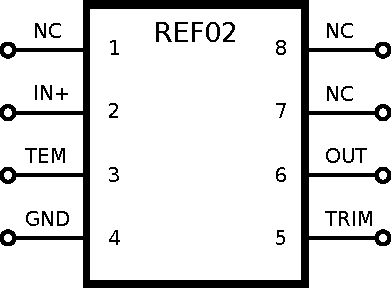
\includegraphics[width=3.5cm]{../E06/latex/REF02.pdf}
%			\caption{Piedinatura dell'integrato\newline REF02.}
%			\label{cir6:REF02}
%	\end{minipage}
\end{itemize}
%\end{figure}
%\vspace{-.8cm}
